\documentclass[UTF8]{ctexart}
% \setcounter{secnumdepth}{1}
\usepackage[a4paper, margin=2cm]{geometry}
\usepackage{chapterbib}
\usepackage{amsmath}
\numberwithin{figure}{section}
\numberwithin{table}{section}
\usepackage{amssymb}
\usepackage{graphicx}
\usepackage{minted}
\usemintedstyle{manni}
\usepackage{subfigure}
\usepackage[colorlinks,linkcolor=orange,anchorcolor=orange,citecolor=orange,urlcolor=black]{hyperref}
\usepackage{pdfpages}
\usepackage[noend]{algpseudocode}
\usepackage{algorithmicx,algorithm}
\usepackage{soul}
\usepackage{xcolor}
\usepackage{booktabs}
\usepackage{caption}
\renewcommand {\thefigure} {\thesection{}-\arabic{figure}}
\renewcommand {\thetable} {\thesection{}-\arabic{table}}
\newcommand{\upcite}[1]{\textsuperscript{\textsuperscript{\cite{#1}}}}
\usepackage{tikz}
\newcommand*\circled[1]{\tikz[baseline=(char.base)]{
            \node[shape=circle,draw,inner sep=0pt] (char) {#1};}}
\renewcommand\bibname{参考文献}
% \pagestyle{plain}
\usepackage{fancyhdr}
\pagestyle{fancy}
\renewcommand{\headrulewidth}{0.4pt}%
\fancyhead[L]{→\_→}
\fancyhead[R]{←\_←}
\fancyhead[C]{欢迎去各大电商平台选购纸质版南瓜书《机器学习公式详解》}
\renewcommand{\footrulewidth}{0.4pt}
\fancyfoot[L]{→\_→}
\fancyfoot[R]{←\_←}
\fancyfoot[C]{配套视频教程:\url{https://www.bilibili.com/video/BV1Mh411e7VU}}
\ctexset{
    section = {
        name = {第,章}
    }
}
\title{南瓜书PumpkinBook}
\author{Datawhale}
\date{2021年2月}

\begin{document}
    \captionsetup[figure]{labelsep=space}
    \captionsetup[table]{labelsep=space}
    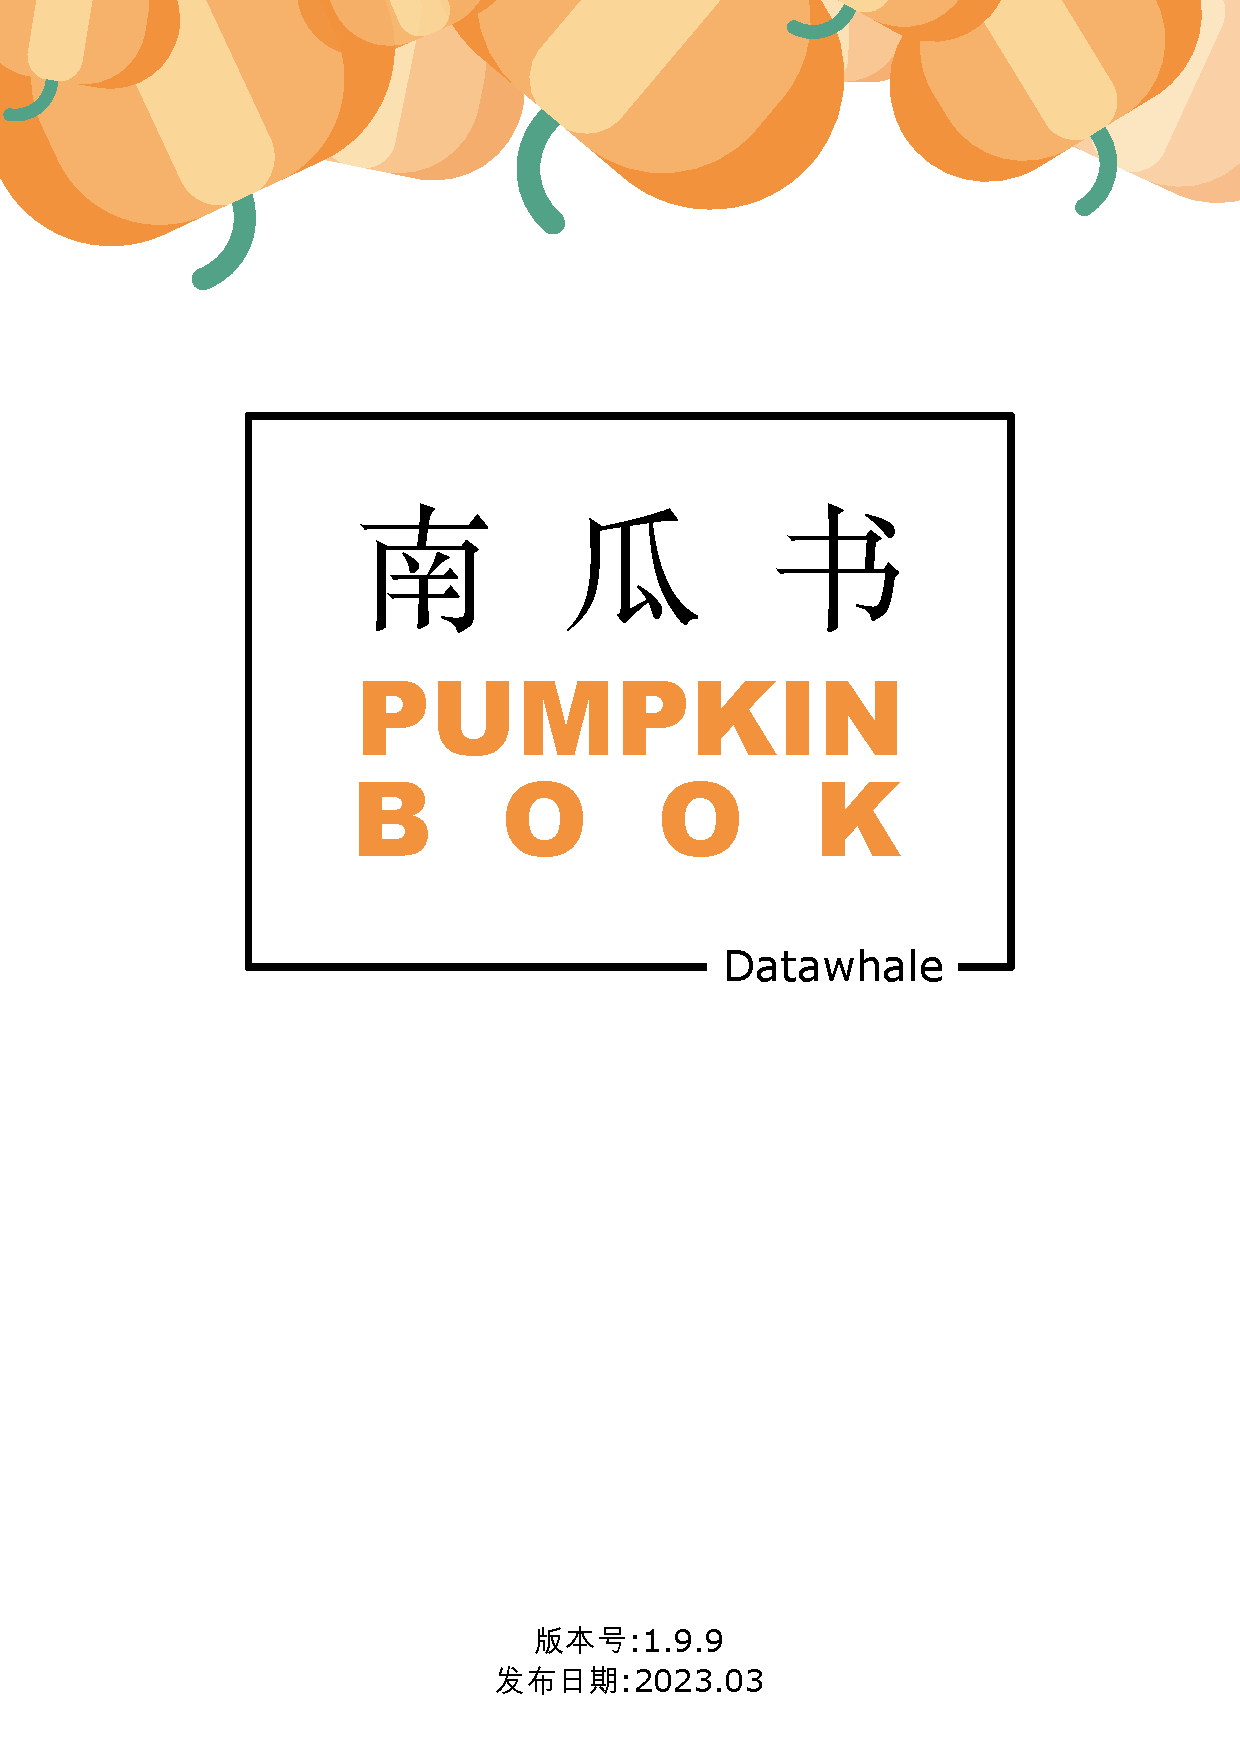
\includepdf[fitpaper=true]{resources/cover.pdf}
    \thispagestyle{empty}
    \clearpage
    
    \section*{前言}
    \renewcommand{\abstractname}{}
    \begin{abstract}
        “周志华老师的《机器学习》(西瓜书)是机器学习领域的经典入门教材之一,周老师为了使尽可能多的读者通过西瓜书对机器学习有所了解, 所以在书中对部分公式的推导细节没有详述,但是这对那些想深究公式推导细节的读者来说可能“不太友好”,本书旨在对西瓜书里比较难理解的公式加以解析,以及对部分公式补充具体的推导细节。”
 
        读到这里,大家可能会疑问为啥前面这段话加了引号,因为这只是我们最初的遐想,后来我们了解到,周老师之所以省去这些推导细节的真实原因是,他本尊认为“理工科数学基础扎实点的大二下学生应该对西瓜书中的推导细节无困难吧,要点在书里都有了,略去的细节应能脑补或做练习”。所以......本南瓜书只能算是我等数学渣渣在自学的时候记下来的笔记,希望能够帮助大家都成为一名合格的“理工科数学基础扎实点的大二下学生”。
        \subsection*{使用说明}
        \begin{itemize}
            \item 南瓜书的所有内容都是以西瓜书的内容为前置知识进行表述的,所以南瓜书的最佳使用方法是以西瓜书为主线,遇到自己推导不出来或者看不懂的公式时再来查阅南瓜书;
            \item 对于初学机器学习的小白,西瓜书第1章和第2章的公式\textbf{强烈不建议深究},简单过一下即可,等你学得有点飘的时候再回来啃都来得及;
            \item 每个公式的解析和推导我们都力(zhi)争(neng)以本科数学基础的视角进行讲解,所以超纲的数学知识我们通常都会以附录和参考文献的形式给出,感兴趣的同学可以继续沿着我们给的资料进行深入学习;
            \item 若南瓜书里没有你想要查阅的公式,或者你发现南瓜书哪个地方有错误,请毫不犹豫地去我们GitHub的Issues(地址:\url{https://github.com/datawhalechina/pumpkin-book/issues})进行反馈,在对应版块提交你希望补充的公式编号或者勘误信息,我们通常会在24小时以内给您回复,超过24小时未回复的话可以微信联系我们(微信号:at-Sm1les);
        \end{itemize}
        \textbf{配套视频教程:}\url{https://www.bilibili.com/video/BV1Mh411e7VU}\\
        \textbf{在线阅读地址:}\url{https://datawhalechina.github.io/pumpkin-book}(仅供第1版)\\
        \textbf{最新版PDF获取地址:}\url{https://github.com/datawhalechina/pumpkin-book/releases}
        \subsection*{编委会}
        \noindent
        \textbf{主编:}Sm1les、archwalker、jbb0523 \\
        \textbf{编委:}juxiao、Majingmin、MrBigFan、shanry、Ye980226 \\
        \textbf{封面设计:}构思-Sm1les、创作-林王茂盛
        \subsection*{致谢}
        特别感谢awyd234、feijuan、Ggmatch、Heitao5200、huaqing89、LongJH、LilRachel、LeoLRH、Nono17、spareribs、sunchaothu、StevenLzq在最早期的时候对南瓜书所做的贡献。
        \noindent
        \begin{center}
        \vspace{1em}
        扫描下方二维码,然后回复关键词“\textbf{南瓜书}”,即可加入“南瓜书读者交流群”\\
        \begin{figure}[hb]
        \centering
        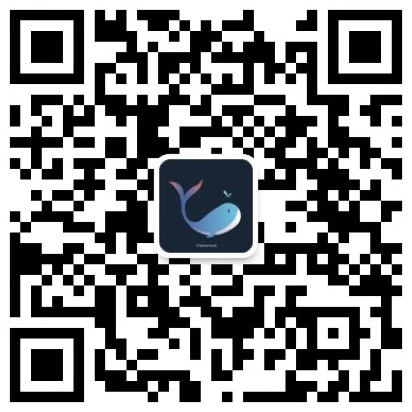
\includegraphics[scale=0.2]{resources/qrcode.jpeg}
        \end{figure}
        \vspace{2em}
        \textbf{版权声明}\\本作品采用\href{http://creativecommons.org/licenses/by-nc-sa/4.0/}{\textbf{知识共享署名-非商业性使用-相同方式共享 4.0 国际许可协议}}进行许可。
        \end{center}
    \end{abstract}
    \thispagestyle{empty}
    \clearpage

    \tableofcontents 
    \thispagestyle{empty}
    \clearpage

    \section{绪论}
\setcounter{page}{1}
这里是一段内容,这里是一段内容,这里是一段内容,这里是一段内容,这里是一段内容,这里是一段内容,这里是一段内容,这里是一段内容,这里是一段内容,这里是一段内容,这里是一段内容,这里是一段内容,这里是一段内容。

这里也是一段内容,这里也是一段内容,这里也是一段内容,这里也是一段内容,这里也是一段内容,这里也是一段内容,这里也是一段内容,这里也是一段内容,这里也是一段内容,这里也是一段内容,这里也是一段内容,这里也是一段内容。

\subsection{引言}
这是2级章节的内容。

\subsubsection{基本术语}
这是3级章节的内容。



\subsection{假设空间}
这里是表\ref{tab.housing-price}的用法。

\begin{table}[H]
    \centering
    \caption{\label{tab.housing-price}房价预测}
    \begin{tabular}{ccc}
        \toprule
        年份&学校数量&房价\\
        \midrule 
        2020&1所&1万/$m^2$\\
        \hline
        2021&2所&4万/$m^2$\\
        \bottomrule
    \end{tabular}
\end{table}

这里是图\ref{fig.roc}的用法。\par
\begin{figure}[h]
\centering
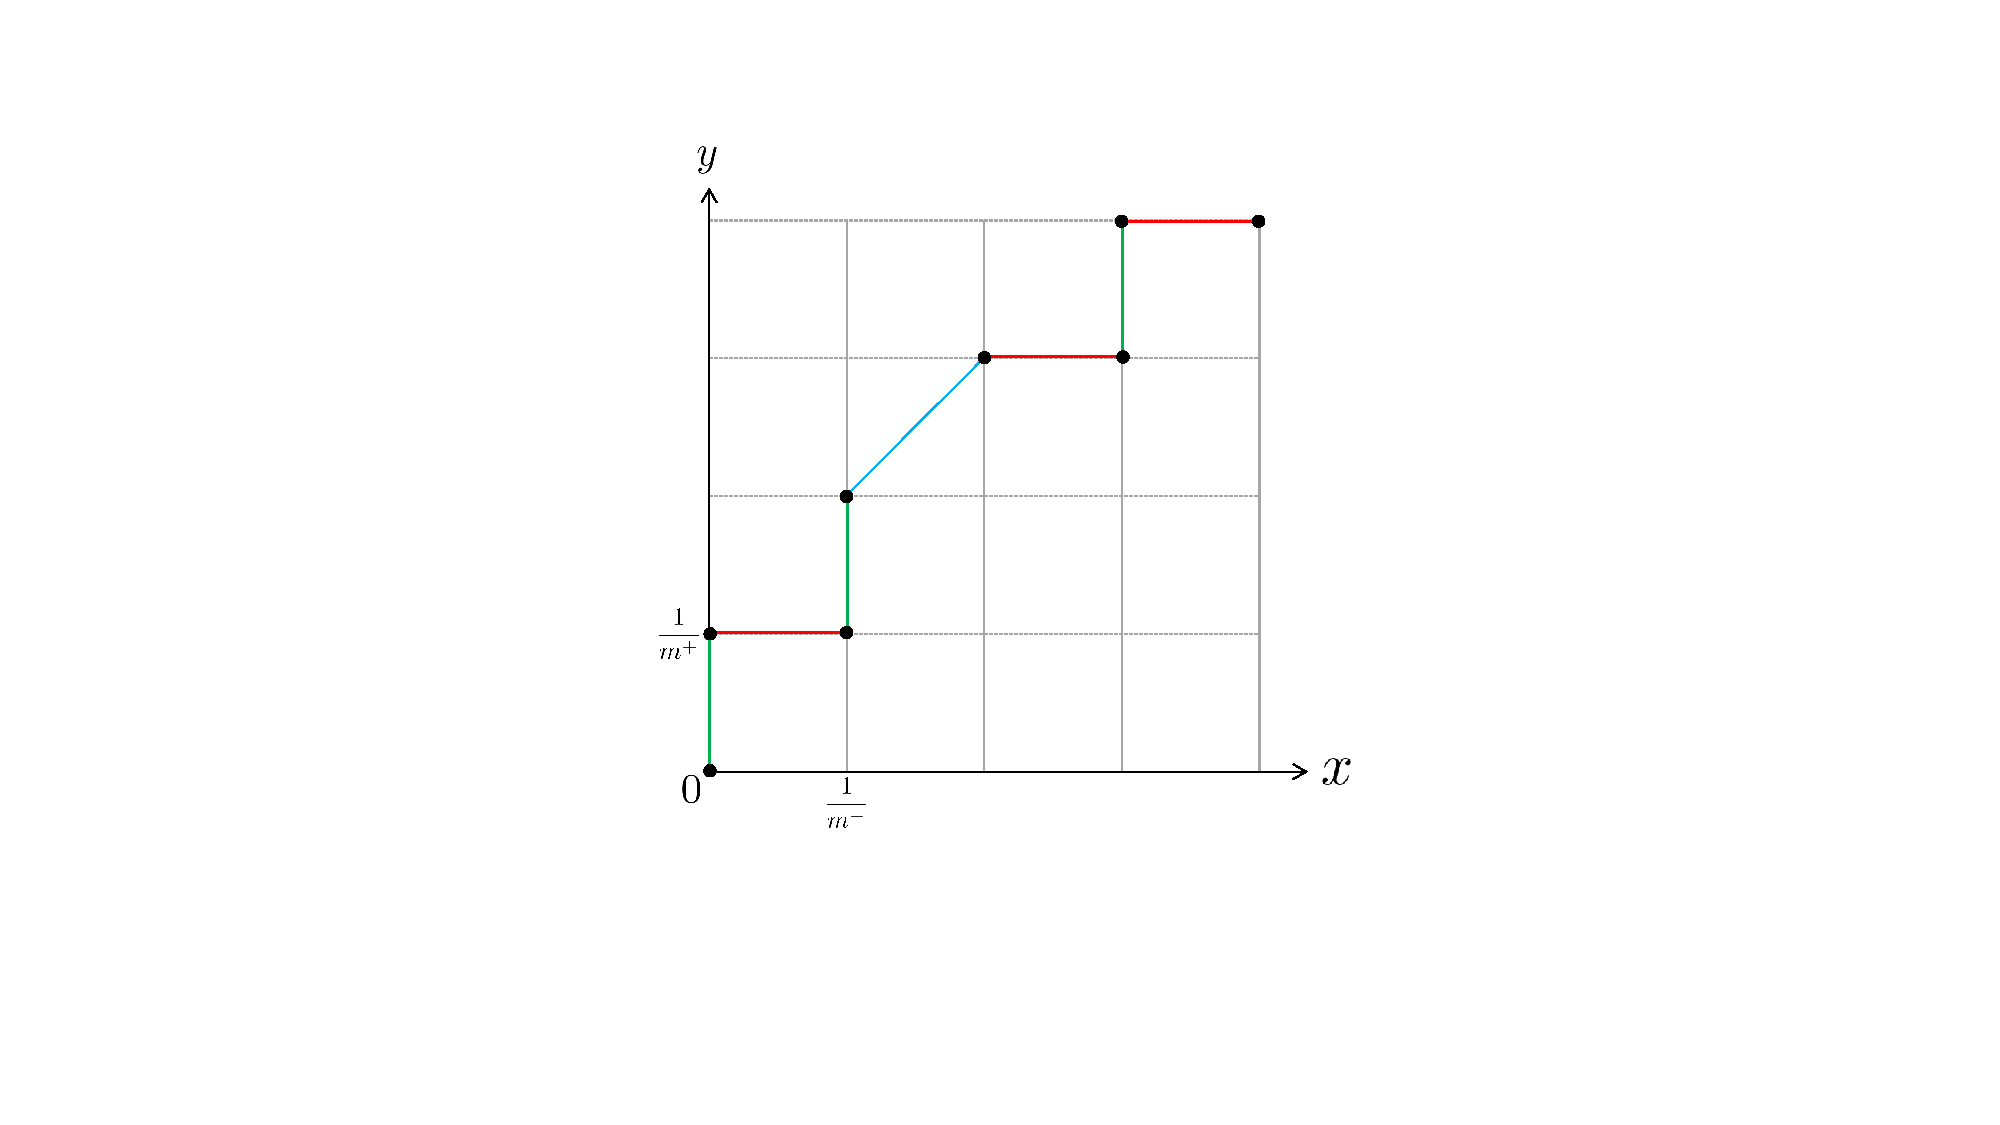
\includegraphics[trim=0 123 0 123,scale=0.5]{resources/ch1/roc.pdf}
\caption{ROC曲线示意}
\label{fig.roc}
\end{figure}

这里是正常引用参考文献\cite{chenxiru},这里是上角标引用参考文献\upcite{chenxiru}。

\bibliographystyle{unsrt}
\bibliography{ref.bib}

\end{document}


